% !TeX root = ../main.tex

\section{Background and Study Design}
\vspace{-3pt}
We present the architecture of a typical task-oriented~dialogue systems, an overview of Rasa, and our study design.

\subsection{Architecture of a Typical Task-Oriented Dialogue System}

A task-oriented dialogue system (TDS) aims to assist~users~in performing specific tasks, such as restaurant booking~and~flight booking~\cite{multiwoz}. 
A pipeline-based TDS consists of four parts,~i.e., natural language understanding (NLU), dialogue state tracking (DST), dialogue policy (Policy) and natural language generation (NLG)~\cite{zhang2020recent}. 
NLU parses a user utterance~into~a~structured~semantic representation, including intent and slot-values.~The~intent is a high-level classification of the user utterance, such as \texttt{Inform} and \texttt{Request}. 
Slot-values are task-specific entities that are mentioned in the user utterance, such as restaurant~price range and location preference. 
After tokenization and featurization of the user utterance, NLU applies classification~models~to recognize intent, and named entity extraction models to extract slot-values. 
DST takes the entire history of the conversation, including both user utterances with predicted intents~and~slot-values and system responses, to estimate the current dialogue state, which is usually formulated as a sequential prediction~task \cite{williams2016dialogstate}.
Dialogue state is typically the probability distribution of user intent and slot-values till the current timestamp.~Given~the estimated dialogue state, Policy generates the next system~action, such as \texttt{Query Database} and \texttt{Utter Question}. 
As Policy determines a series of actions sequentially, sequential models such as Recurrent Neural Network (RNN) are applied. 
For actions that require a response, NLG converts the action into a natural language utterance, which is often considered as a sequence generation task~\cite{wen-etal-2015-semantically}.


\subsection{An Overview of Rasa 3.0}\label{sec:rasa_overview}

Rasa is a popular open-source ML-enabled TDS, which~is fully implemented with Python and used by many well-known companies in customer service for real users, including Adobe, Airbus, and N26 \cite{rasa}. 
An architecture overview~of~Rasa 3.0 is shown in Fig. \ref{overview_fig}. %A \textit{module} serves as a semantic function to transform given input into specific output, while 
Each module consists of one single component or multiple semantically similar components. 
%For example, there are multiple components inside \textit{Policy} module, which is implemented with ML models or rule-based code logic to predict the next system action. 
Apart from the modules in a typical TDS, Rasa proposes the Selector~module~to select candidate intents and responses for FAQ questions~\cite{chaudhuri-etal-2018-improving}.
We present some concepts in Rasa 3.0 to ease our presentation.

\textbf{Components in Rasa.} There are two types of components~in Rasa. We define \textit{ML components}~as~components that~are~implemented with ML models, and \textit{rule-based components} as components that are implemented with rule-based code logic.
General utils code in Rasa is not considered in this paper, such as command line and database access code.
% We consider rule-based components in this paper, because there may exist interactions between them and ML components. As a complex ML-enabled system, there exists inter-module and intra-module interactions among themselves, and a series of data processing code before and after the model usages within each component.

\textbf{Configuration File and Component Graph in Rasa.}~As there are multiple available components~in~each~module,~developers need to choose components that are actually used~in the Rasa pipeline with a \textit{configuration file} to build a chatbot. 
Parameters of each component~are~specified~in~the~configuration file (e.g., ML model used by a component~and hyperparamers of a ML model).
Rasa applies Dask~\cite{dask} to compile~a~configuration file into a component graph. 
Each node in the component~graph denotes a component, and the edges connected with it denote upstream and downstream components with input and output data dependency. 
Execution of components obeys~the~topological order specified by edges.
These components interact with each other through fields in shared \texttt{Message} class instances. %including \texttt{Message.sequence\_features}, \texttt{Message.intent} and \texttt{Message.entities}.
An upstream component stores outputs to \texttt{Message} instances, and a downstream component retrieves them for further processing. 

\textbf{ML Stages in Rasa.} 
Different from Apollo, which uses trained model files from external systems, and therefore~only contains the inference stage of ML models \cite{pengFirstLookIntegration2020}, the training, evaluation and inference stages of ML models are all~present in Rasa. 
Given a configuration file, Rasa separately compiles it to a training component graph and~an~inference~component graph. 
% which specify the methods in components that should be invoked in these stages.
In training stage, the trainable~upstream~components are first trained, and then process the training data used by downstream components. 
%For example, the \textit{CountVectorsFeaturizer} component is trained first, and then the \texttt{process\_training\_data} of it is called to create features for classifiers to be traind.
In evaluation stage, only the performance metrics of \textit{IntentClassifier}, \textit{EntityExtractor} and \textit{Policy} are reported, as there is no ground truth for evaluation data in other modules.


%\textbf{Test Cases in Rasa.} 
%Rasa provides a test suite of~47~test files and 461 test functions for ML-related code. We consider each test function as a test case. These test cases target at different granularity levels, including method-level, component-level and integration-level.
%There are four types of test oracles, including given input-output pairs, component-specific constraints, differential executions and exception oracles. 
%All three previously mentioned ML stages are tested.
%To test the training stage of a component, test cases must first train it  and check whether any test oracle is violated.
%The statistics of test cases are presented in Section \ref{sec:test_case}.


\subsection{Study Design}

Our goal is to understand the complexity and its impact on testing in Rasa. To achieve this goal, we propose five RQs. %the first three research questions to characterize the complexity at three levels and the last two research questions to investigate its impact on testing as follows.

\begin{itemize}[leftmargin=*]
    \item \textbf{RQ1 System Complexity Analysis}: how ML components~are adopted across the modules in Rasa?
    \item \textbf{RQ2 Interaction Complexity Analysis}: how ML components interact with other~components in Rasa?
    \item \textbf{RQ3 Component Complexity Analysis}: how the code of ML components is composed by what kinds~of~code?
    \item \textbf{RQ4 Testing Practice Analysis}: how is the characteristic of test cases, and how well~they cope with the complexity?
    \item \textbf{RQ5 Mutation Testing Analysis}: how~is~the~bug-finding capability of test cases and test data (i.e., the data for testing models), and how well they cope with the complexity?
\end{itemize}

\textbf{RQ1} aims to identify ML components in Rasa and broadly view them from the perspective of dependent libraries and ML models. 
\textbf{RQ2} aims to summarize a comprehensive taxonomy of component interaction patterns. 
\textbf{RQ3} aims to inspect the source code inside every component to characterize the statistics and composition patterns of different code types, including data processing code, model usage code, etc. 
Our findings from \textbf{RQ1}, \textbf{RQ2} and \textbf{RQ3} could reveal how the complexity originates and manifests in real world large-scale ML-enabled systems, which provide both practitioners and researchers with insights to overcome the complexities involved in implementing, maintaining, debugging and testing such complex systems. 

\textbf{RQ4} aims to quantitatively assess Rasa's test cases from~code coverage, test case statistics (i.e., granularity levels, oracle~types, and ML stages), and component interaction coverage perspectives. 
\textbf{RQ5} aims to generate mutants (i.e., artificial bugs) and check whether these mutants can be killed (i.e., detected) by test cases. 
Further, for the survived mutants, we train~Rasa~with 3 default configuration files on \textit{MutiWoz} \cite{multiwoz}, a widely used multi-domain TDS dataset. 
We calculate the statistical significance between the performance metrics from mutated Rasa code with metrics from pipelines trained with clean code.
Our findings from \textbf{RQ4} and \textbf{RQ5} evaluate the testing practice in Rasa, and shed light on automated test generation, bug localization and bug repairing techniques for complex ML-enabled systems.


\begin{figure*}[!t]
\centering
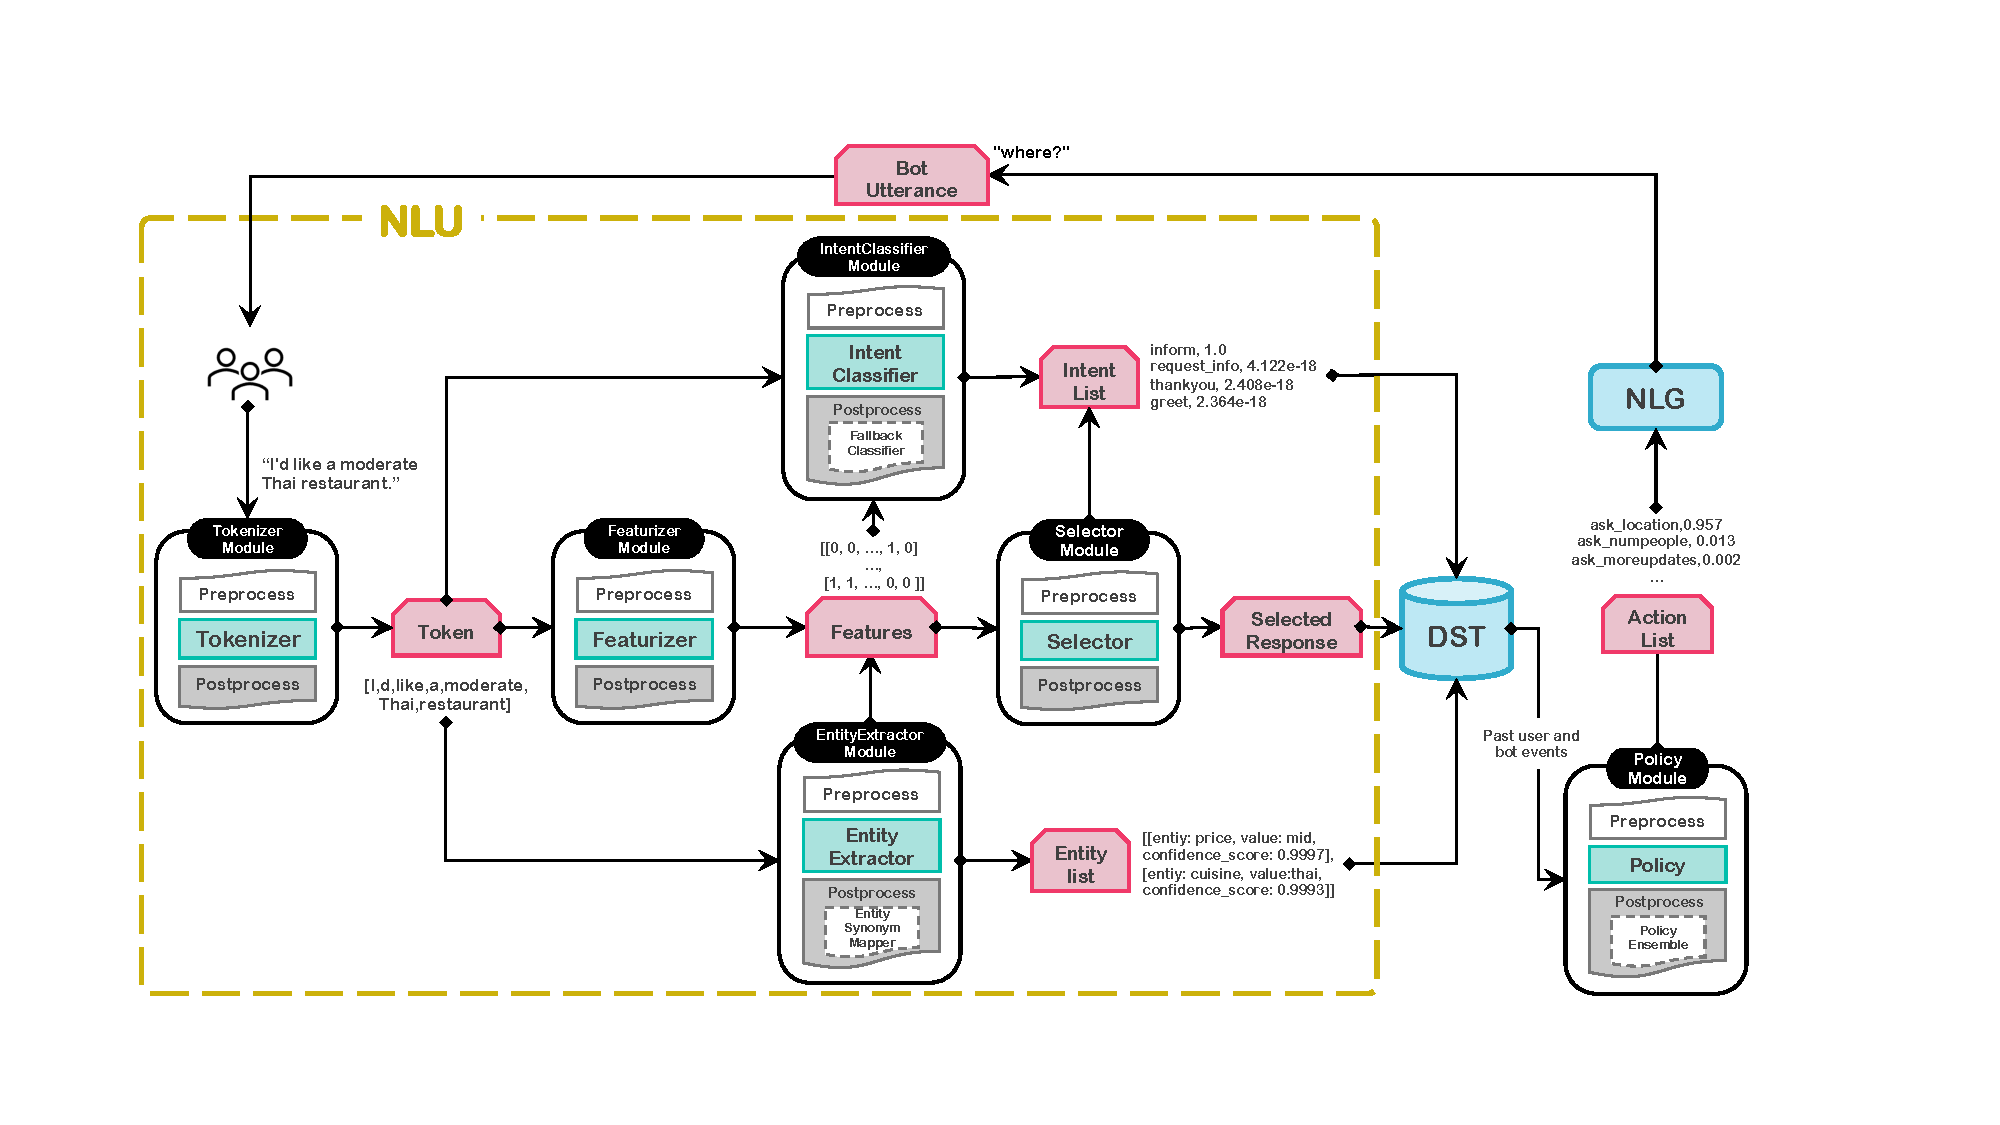
\includegraphics[scale=0.60]{figs/overview.pdf}
\caption{The Modules and Workflow of Rasa}\label{overview_fig}
\end{figure*}

\begin{table*}[!h]
	\caption{System Complexity Analysis of Rasa}
	\vspace{-10pt}
	\begin{center}
        \scalebox{0.97}{
	\begin{tabular}{llllllllll}
	\toprule
	\textbf{Module}
	& \textbf{Component}
	& \textbf{Direct Lib.}
	& \textbf{Indirect Lib.}
	& \textbf{Model Type}
	& \textbf{No. Model}
    & \textbf{Trainable}
    & \textbf{Rasa Imp.}
    & \textbf{LoC}\\
	\midrule
	\multirow{4}*{Tokenizer}
	&\cellcolor{Gray}JiebaTokenizer & \cellcolor{Gray}Jieba &\cellcolor{Gray}N/A &\cellcolor{Gray}HMM & \cellcolor{Gray}1 &\cellcolor{Gray}False  &\cellcolor{Gray}False   &\cellcolor{Gray}85  \\
	&\cellcolor{Gray}SpacyTokenizer &\cellcolor{Gray}Spacy &\cellcolor{Gray}Thinc &\cellcolor{Gray}MLP &\cellcolor{Gray}1 &\cellcolor{Gray}False  &\cellcolor{Gray}False &\cellcolor{Gray}39  \\
	&MitieTokenizer &Mitie &N/A &N/A &N/A &False  &False &43  \\
    &WhitespaceTokenizer &N/A &N/A &N/A &N/A &False &True &52    \\
	\midrule
	\multirow{7}*{Featurizer}
	&\cellcolor{Gray}ConveRTFeaturizer &\cellcolor{Gray}TensorFlow &\cellcolor{Gray}N/A &\cellcolor{Gray}Transformer &\cellcolor{Gray}1 &\cellcolor{Gray}False &\cellcolor{Gray}False &\cellcolor{Gray}269 \\
	&\cellcolor{Gray}LanguageModelFeaturizer &\cellcolor{Gray}Transformers &\cellcolor{Gray}TensorFlow &\cellcolor{Gray}Transformer &\cellcolor{Gray}6 &\cellcolor{Gray}False &\cellcolor{Gray}False &\cellcolor{Gray}378  \\
	&\cellcolor{Gray}MitieFeaturizer &\cellcolor{Gray}Mitie &\cellcolor{Gray}Dlib &\cellcolor{Gray}CCA &\cellcolor{Gray}1 &\cellcolor{Gray}False &\cellcolor{Gray}False &\cellcolor{Gray}98   \\
    &\cellcolor{Gray}SpacyFeaturizer &\cellcolor{Gray}Spacy &\cellcolor{Gray}Thinc &\cellcolor{Gray}CNN &\cellcolor{Gray}2 &\cellcolor{Gray}False &\cellcolor{Gray}False &\cellcolor{Gray}66   \\
    &CountVectorsFeaturizer &Scikit-learn &N/A &N/A &N/A &True &False &520   \\
    &LexicalSyntacticFeaturizer &N/A &N/A &N/A &N/A &True  &True &319  \\
    &RegexFeaturizer &N/A &N/A &N/A &N/A &True &True &151  \\
    \midrule
    \multirow{5}*{IntentClassifier}
    &\cellcolor{Gray}DIETClassifier &\cellcolor{Gray}TensorFlow &\cellcolor{Gray}N/A &\cellcolor{Gray}Transformer &\cellcolor{Gray}1 &\cellcolor{Gray}True &\cellcolor{Gray}True &\cellcolor{Gray}1217 \\
    &\cellcolor{Gray}MitieIntentClassifier &\cellcolor{Gray}Mitie &\cellcolor{Gray}Dlib &\cellcolor{Gray}SVM &\cellcolor{Gray}1 &\cellcolor{Gray}True &\cellcolor{Gray}False &\cellcolor{Gray}89 \\
    &\cellcolor{Gray}SklearnIntentClassifier &\cellcolor{Gray}Scikit-learn &\cellcolor{Gray}N/A &\cellcolor{Gray}SVM &\cellcolor{Gray}1 &\cellcolor{Gray}True &\cellcolor{Gray}False &\cellcolor{Gray}173 \\
    &FallbackClassifier  &N/A &N/A &N/A &N/A &False &True&91   \\
    &KeywordIntentClassifier  &N/A &N/A &N/A &N/A &True &True&132  \\
    \midrule
    \multirow{7}*{EntityExtractor}
    &\cellcolor{Gray}DIETClassifier &\cellcolor{Gray}TensorFlow &\cellcolor{Gray}N/A &\cellcolor{Gray}Transformer &\cellcolor{Gray}1 &\cellcolor{Gray}True &\cellcolor{Gray}True &\cellcolor{Gray}1217 \\
    &\cellcolor{Gray}CRFEntityExtractor &\cellcolor{Gray}Scikit-learn &\cellcolor{Gray}N/A &\cellcolor{Gray}CRF &\cellcolor{Gray}1 &\cellcolor{Gray}True &\cellcolor{Gray}False &\cellcolor{Gray}438 \\
    &\cellcolor{Gray}MitieEntityExtractor &\cellcolor{Gray}Mitie &\cellcolor{Gray}Dlib &\cellcolor{Gray}SVM &\cellcolor{Gray}1 &\cellcolor{Gray}True &\cellcolor{Gray}False &\cellcolor{Gray}164 \\
    &\cellcolor{Gray}SpacyEntityExtractor  &\cellcolor{Gray}Spacy &\cellcolor{Gray}Thinc &\cellcolor{Gray}MLP &\cellcolor{Gray}1 &\cellcolor{Gray}False  &\cellcolor{Gray}False &\cellcolor{Gray}52  \\
    &DucklingEntityExtractor  &N/A &N/A &N/A &N/A &False &False &134   \\
    &RegexEntityExtractor &N/A &N/A &N/A &N/A &True  &True &124  \\
    &EntitySynonymMapper &N/A &N/A &N/A &N/A &True  &True &102  \\
    \midrule
    Selector
    &\cellcolor{Gray}ResponseSelector &\cellcolor{Gray}TensorFlow &\cellcolor{Gray}N/A &\cellcolor{Gray}Transformer &\cellcolor{Gray}2 &\cellcolor{Gray}True &\cellcolor{Gray}True &\cellcolor{Gray}560  \\
    \midrule
    \multirow{6}*{Policy}
    &\cellcolor{Gray}TEDPolicy &\cellcolor{Gray}TensorFlow &\cellcolor{Gray}N/A &\cellcolor{Gray}Transformer+CRF &\cellcolor{Gray}1 &\cellcolor{Gray}True &\cellcolor{Gray}True &\cellcolor{Gray}1262 \\
    &\cellcolor{Gray}UnexpecTEDIntentPolicy &\cellcolor{Gray}TensorFlow &\cellcolor{Gray}N/A &\cellcolor{Gray}Transformer+CRF &\cellcolor{Gray}1 &\cellcolor{Gray}True &\cellcolor{Gray}True &\cellcolor{Gray}458 \\
    &MemoizationPolicy &N/A &N/A &N/A &N/A &True &True &207   \\
    &AugmentedMemoizationPolicy &N/A &N/A &N/A &N/A &True &True &65   \\
    &RulePolicy &N/A &N/A &N/A &N/A &True &True &818   \\
    &PolicyEnsemble &N/A &N/A &N/A &N/A &False &True &150   \\
	\bottomrule
	\end{tabular}		
	\label{system_complexity}}
	\end{center}
\end{table*}
